\section{Introduction}

\lettrine[lines=2]Music, especially in the form of song, is ubiquitous across human societies. Although some features of music are considered universal---songs are dominated by short phrases, discrete pitches with small melodic intervals, and simple rhythmic ratios \autocite{mehr2019, savage2015}---there exists significant variation that is specific to different cultural traditions, times, and places. This diversity emerges from a complex interplay between cognitive and motor factors common to all humans, which anchors variation, with the dynamics of exposure and preference, transmission errors, and other neutral processes that lead, over time, to cultural divergence \autocite{tchernichovski2017,verhoef2021,tierney2011,savage2019,savage2019} 

Songs are typically passed down orally, and this process of learning and reproduction introduces changes in their structure; some random, and others directional. However, these learning and cultural transmission processes do more than just introduce minor variations in pitch or timing; they can also shape the underlying structure of melody and rhythm, pushing them toward stable musical 'cultural attractors' \autocite{claidiere2007, buskell2017}. These attractors manifest as relatively discrete modes within the distribution of melodic and rhythmic intervals \autocite{anglada-tort2023, verhoef2021, jacoby2021}, which may serve to align the perception, memory, and reproduction of information between individuals, enhancing the fidelity of cultural transmission and limiting the drift of cultural traits \autocite{anglada-tort2023, heyes2018a, feher2009, saldana2019, trehub2015, falandays2022}.

Recent findings suggest that similar processes may take place in the songs of certain bird species that exhibit structured, categorical organisation in their songs. For example, \textcite{roeske2020} found that domestic zebra finch \textit{Taeniopygia guttata} and thrush nightingale \textit{Luscinia luscinia} songs had discretised isochronous rhythms. \textcite{xing2022} describe that Australian pied butcherbird \textit{Cracticus nigrogularis} rhythms are categorically organised, and the songs of hermit thrushes \textit{Catharus guttatus} \autocite{doolittle2014} and musician wrens \textit{Cyphorhinus arada} \autocite{doolittle2012} use notes whose frequencies are related by small intervals in the overtone series (but see exceptions: \cite{araya-salas2012, dobson1977}). This has been interpreted as evidence that some basic characteristics of human music might arise through processes that are more taxonomically widespread \autocite{doolittle2014}.

It is essential to recognise that, while human music and bird song are often compared, they are far from perfect analogues; they serve different purposes and are subject to distinct evolutionary pressures. Birdsong, in particular, is much more constrained due to factors such as sexual selection, energy costs, and the different species' ecology \autocite{verzijden2012, demery2021, nowicki1998, spencer2003, sierro2023}. Nevertheless, there are significant parallels between human and songbirds' vocal learning capabilities and the neural circuitry that underlies them, which has led to the establishment of songbirds as a model system in the study of vocal learning \autocite{jarvis2019, rouse2021}. Our current understanding suggests that bird species capable of vocal learning have a genetically predetermined 'song space' \autocite{james2017, lachlan2010}; within it, and paralleling human cultural variation, songs can evolve in various directions due to demographic and cultural processes. In this sense, it is reasonable to speculate that some of the same mechanisms that give rise to 'cultural attractors' enhancing the fidelity of song transmission in human cultures may also operate in bird songs. These mechanisms, as discussed by \autocite{tchernichovski2017}, likely include a compression process that leads to the transition from continuous variation to categorical syllable types---a phenomenon similar to that described in the evolution of linguistic structure \autocite{gibson2019, decastro-arrazola2019, kirby2017, tamariz2016, silvey2019}. This transition could result from motor and perceptual biases or the dynamics of cultural transmission itself, both of which could contribute to more accurate song transmission.

This leads to the intriguing possibility that cultural stability in bird song across larger temporal and spatial scales may not solely result from accurate learning, as assumed in most models of song evolution \autocite{lachlan2018, hudson2022, pichkar2023, youngblood2022}. Instead, underlying structural biases similar to those present in music and language may play an important role. The presence of stable structural patterns in bird songs could shed light on the seemingly paradoxical nature of cultural change in species where song cultures exhibit polymorphism, experience significant and rapid turnover of cultural variants, and yet adhere to recognizable and stable patterns over long time periods. To explore these questions, rather than focusing on concrete acoustic features such as spectral bandwidth, fundamental frequency, or note duration, we need to move on to study the relational properties underpinning songs---their melodic and rhythmic structure. We aim a) to determine whether these structural aspects exhibit clustering within the song space of species and, if so, b) to what extent attractor points or regions of high probability can themselves vary culturally. 

This chapter tackles the first of these questions, which regards the distribution of melodic and rhythmic structure in bird songs. To do this, we use a dataset comprising more than a million notes from a population of great tits, collected over three years in Wytham Woods, Oxfordshire, UK \autocite{merinorecalde2023a}. While great tits may not be celebrated for their melodious tunes, with some likening their songs to a 'squeaky wheelbarrow' or 'bicycle pump', they are great for this research: their songs consist of phrases composed of one to three spectrally simple and stable notes, which restricts their combinatorial complexity and allows automated analysis. Our preliminary findings provide evidence that the melodic and rhythmic landscape of great tit songs exhibits a high degree of structure, suggestive of sources of stability beyond accurate learning of song types.

\section{Methods}
\label{c5:methods}

\autoref{chapter:3} contains a detailed description of the data collection and preparation process, and \autoref{c3_fig:pipeline} shows a graphical description. \figref[a]{c5_fig:methods} contains a visual summary of the melodic interval and rhythmic ratio extraction process.

\subsection{Study site and data collection}
We study great tits, small birds with a short reproductive lifespan of around 1.9 years. These birds sing often during the breeding season, which lasts from March to June. They form socially monogamous pairs and defend territories around their nests \parencite{hinde1952}. We carried out this research Wytham Woods, in Oxfordshire, UK (51\degree46 N, 1\degree20 W). This semi-natural deciduous woodland spans approximately 385 hectares and has been under study since 1947 \parencite{lack1964}. Most great tits in this population breed in marked nest boxes, with individuals bearing unique British Trust for Ornithology (BTO) metal leg rings. Our data collection spanned from late March to mid-May in the breeding seasons of 2020, 2021, and 2022. Fieldworkers regularly checked the 1018 great tit nest boxes weekly before and during the egg-laying period, recording information such as breeding pair identities, clutch initiation and egg-hatching dates, clutch size, and fledgling number.

To capture male great tit vocalisations, we took advantage of the bird's behaviour during the reproductive period, when they consistently sing near their nests at dawn, before and during egg-laying \parencite{mace1987}. We deployed autonomous AudioMoth \autocite{hill2019} sound recorders near nest boxes occupied by great tits, placing them on nearby trees at a consistent height and orientation (within 1 to 2 metres of the nest box and no more than 5 metres away). We used 60 AudioMoth recorders (30 in 2020), housed within custom waterproof enclosures. Our recording sessions began approximately one hour before sunrise, (sunrise times during the recording period spanned from 05:36 to 04:00 UTC). Each session consisted of seven consecutive 60-minute recordings, sampled at 48 kHz with a 16-bit depth. To cover a wide range of bird activity, we placed each recorder at a single location for at least three consecutive days before relocating it to a different nest box. This involved moving 20 recorders daily (10 in 2020) across the study site. Despite variations in song amplitude due to distance and direction, our observations didn't reveal any systematic bias in song selection.

\subsection{Ethical note}
All work involving birds was subject to review by the University of Oxford, Department of Zoology, Animal Welfare and Ethical Review Board (approval number: \nolinkurl{APA/1/5/ZOO/NASPA/Sheldon/TitBreedingEcology}). Data collection adhered to local guidelines for the use of animals in research and all birds were caught, tagged, and ringed by BTO licence holders (NMR's licence: C/6904).

\subsection{Data processing and annotation}

We processed and annotated the recordings using custom software and Python 3 scripts \parencite{vanrossum1995}, with the open-source package \texttt{pykanto} \parencite{merinorecalde2023}. The tools and scripts can be accessed at \href{https://github.com/nilomr/great-tit-hits-setup}{\nolinkurl{github.com/nilomr/great-tit-hits-setup}}. 

\noindent In our data processing workflow, we began by segmenting songs based on visual inspection of spectrograms, aiming to isolate segments where bird notes were distinctly discernible from background noise. This manual process was performed using Sonic Visualiser \parencite{cannam2010}. To ensure that songs were correctly attributed to individual birds, we implemented measures to minimise false positives. Recordings with multiple vocalising birds were discarded unless one bird's vocalisation was significantly louder. Songs with a maximum amplitude below a threshold of -16 dB were also discarded (see \cite{merinorecalde2023a}). We used normalised, band-passed mel-scale spectrogram representations for all subsequent operations (specific parameters detailed in the repository \href{https://github.com/nilomr/great-tit-hits-setup}{repository}).

\subsubsection{Note segmentation}

Next, we segmented songs into their constituent notes using a dynamic threshold algorithm implemented in pykanto \parencite{merinorecalde2023}, partly based on work by \textcite{sainburg2019}. After a series of morphological transformations and de-echoing, the algorithm identified spectral envelope minima as silences and divided the signal into shorter segments when needed, while discarding segments below minimum note duration.
This relatively naive automated segmentation process is sensitive to factors like background noise, varying note amplitude, vegetation interference, sound direction changes, and performance variations, which can lead to missed or incorrectly delimited notes. Despite these challenges, we achieved an estimated 96.3\% accuracy based on manual checks of 1048 randomly selected notes.

\subsubsection{Song type annotation}

Finally, we classified each song type in the dataset using a semi-supervised approach implemented in \texttt{pykanto}. This involved creating average unit spectrograms for each song, reducing dimensionality with UMAP \parencite{mcinnes2018}, and performing cluster analysis with HDBSCAN \parencite{mcinnes2017} for each bird. While useful, this method can sometimes separate similar song renditions due to performance variation or background noise, potentially overestimating the repertoire size. To mitigate this, we employed \texttt{pykanto}'s interactive app to review and adjust clusters as needed \cite{merinorecalde2023a}. We benefited from the consistent songs of great tits, which have relatively limited, stereotyped repertoires (1 to fewer than 15 song types).

\subsection{Calculating rhythmic and melodic structure}


\subsubsection{Melodic intervals}

First, for each note segment, we convert onset and offset times in seconds to frame indices, extract the corresponding audio segments and compute the Short-Time Fourier Transform. Then, we apply a binary frequency mask to the magnitude spectrogram to retain only the frequencies within a specified range ($f_{min}$ to $f_{max}$), determined by the region of interest in the frequency domain drawn during segmentation. We then compute the mean of the masked spectrogram along the frequency axis to obtain the mean magnitude for each frequency bin and identify the one with the maximum value as the peak frequency. Great tit songs are spectrally simple, so this provides a good estimate in most cases.

\noindent After this, we calculate the interval size for each pair of adjacent note frequencies in the song,

\begin{equation}
\Delta_{ST} = 12 \cdot \log_2\left(\frac{f_{i}}{f_{i+1}}\right)
\end{equation}

\noindent Where $\Delta_{ST}$ represents the semitones difference between two consecutive note frequencies, $f_{i}$ is the frequency of the $i$-th note, and $f_{i+1}$ is the frequency of the $i+1$-th note.


\paragraph{Strength of interval categories}
\label{c5:strength}
For clarity, we partition our analyses based on the spectral properties of notes in a song (see \nameref{c5:typology}). The pure, stable-tone tone melodies typically preferred in studies of bird songs \autocite{dobson1977, tierney2011a, doolittle2012, doolittle2014} show strong evidence of interval categories, which cannot be attributed to poor sampling (this is the second most common category, with n = 28,542) or an artefact of the frequency extraction process (we can resolve differences $>$ 21.5 Hz). Although the position of the modes in the distributions derived from all other 2-note types is similar, we still need to make sure that the weaker pattern found in songs where notes are spectrally more complex (e.g., have harmonics) is not an artefact of the frequency extraction process and indeed reflects looser categories.

\subsubsection{Rhythmic intervals}

We calculated song rhythmic ratios, denoted as $R$, as the ratio of each interval to the total length of that interval along with the subsequent one, following \textcite{roeske2020, xing2022}:

\begin{equation}
R = \frac{i_{n}}{i_{n} + i_{n+1}}
\end{equation}

\noindent Here, $i_{n}$ stands for the Inter-Onset Interval between the $n$-th note and the next note ($n+1$). Each Inter-Onset Interval ($IOI_i$) is calculated from the time segmentation described in the previous section as:

\begin{equation}
IOI_i = Onset_{i+1} - Onset_i
\end{equation}

\noindent Where $i$ ranges from 1 to $n-1$, representing each note except the last one.

\begin{figure*}[hb!]
    \centering
    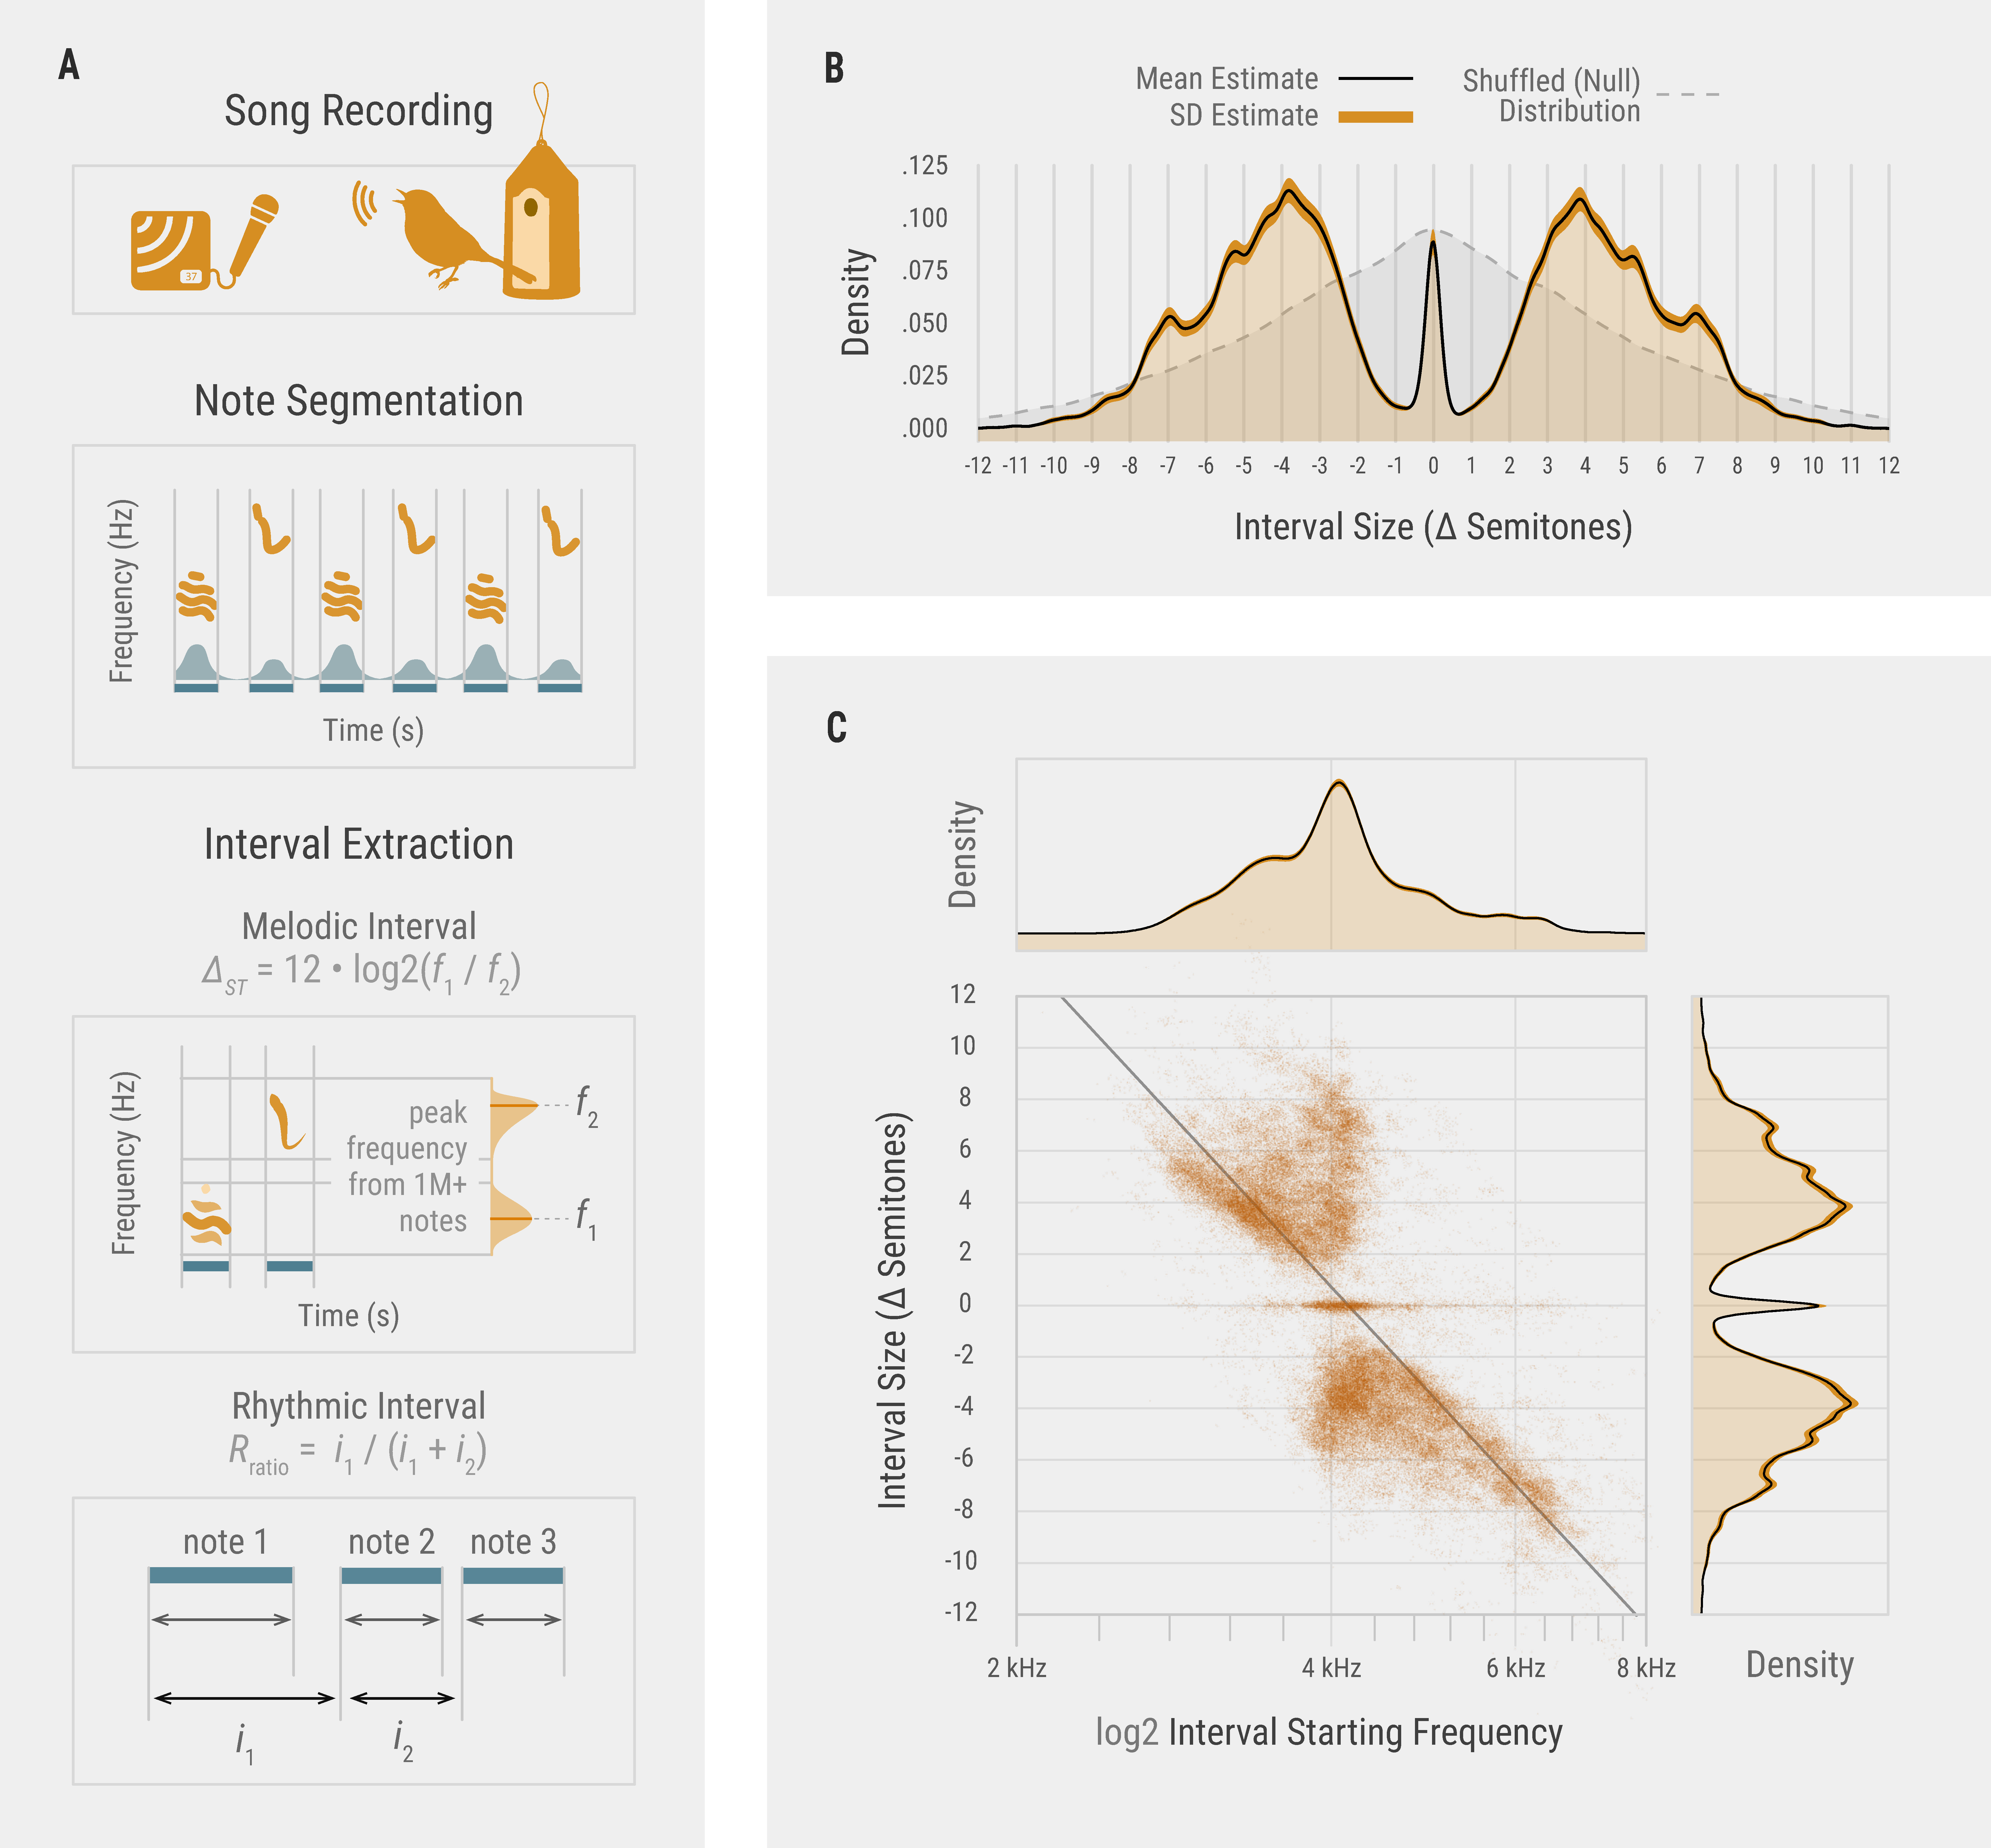
\includegraphics[width=\linewidth]{figures/chapter_5/methods-melodic-null.pdf}
    \mycaption{Visual description of the methods; melodic structure in great tit songs}{
        (A) Simplified visual summary of the process used to extract melodic and rhythmic intervals; see also \nameref{c5:methods}
        (B) Density estimate of the distribution of interval sizes over the entire dataset (songs consisting of two notes), with mean (black line) and SD (orange line). The discontinuous grey line represents a null distribution created by shuffling the empirical distribution of frequencies and recalculating interval sizes. It represents the expected distribution if birds with the same motor-vocal constraints did not have a preference for interval sizes within their range.
        (C) Great tit songs strongly show a pattern known as skip-reversal, where larger intervals are associated with extreme pitches, which has been the subject of debate in (human) musicology \autocite{vonhippel2000} but likely arises from a simple process of regression to the mean.
    }
    \label{c5_fig:methods}
\end{figure*}

\subsubsection{Resampling and Kernel Density Estimation}

Songs have varying lengths, and levels of vocal production by birds differ greatly. To ensure that our results were not driven by an imbalance in the data, we sampled 5 intervals with replacement from each song sung by each bird, then repeated this process for each song type, so that each song type contributed 10 songs to the balanced dataset. Finally, to account for variation in repertoire size and sample size per year, we again sampled songs with replacement from each individual bird or year, depending on the analysis, during the Kernel Density Estimation (KDE) procedure.

To explore the distribution of melodic interval sizes and rhythmic ratios, following \textcite{anglada-tort2023} we compute one-dimensional KDEs over a grid of 1000 values in the the range of the data, using a bandwidth of 0.15 semitones for melodic intervals and 0.015 s for the rhythmic intervals to balance smoothing and resolution. Then, to quantify uncertainty around the mean KDE estimates, we bootstrap them by repeatedly resampling the data, recomputing the KDE, and calculating the mean and standard deviation of the density estimate across the bootstrap samples. We do this for the entire dataset, and for each in the typology of songs described below separately.


\subsubsection{Song typology}
\label{c5:typology}
To investigate potential variations in the motor challenges and constraints associated with different song types, we classified songs into distinct subsets based on the number of notes, spectral properties of the notes, and the presence or absence of frequency modulation, defining the following song typology (sample sizes in the balanced dataset in parenthesis):

\begin{itemize}
    \item \textbf{One note}: Songs consisting of a single note repeated rhythmically
    \item \textbf{Two notes}: All songs composed of two different, alternating notes.
    \item \textbf{Two notes, pure and unmodulated}: Songs with two notes, each consisting of a single stable, pure, unmodulated tone.
    \item \textbf{Two notes, none pure}: All two-note songs where neither note is pure and unmodulated
    \item \textbf{Two notes, both harmonic}: Songs featuring two notes, both of which have harmonic components.
    \item \textbf{Three or more notes}: Songs comprising three or more notes. There are few three-note melodies, so we did not split these by spectral or modulation properties.
\end{itemize}

\noindent Because we are extracting dominant or peak frequencies $f_d$ instead of fundamentals $f_0$, there is a chance that the results for songs with notes that are not pure-tone or where $f_d$ and $f_0$ do not coincide are noisier, or do not capture the target pitch as well. This typology also allows us to isolate songs made up of pure-tone notes, which have been preferentially used in prior work \autocite{dobson1977, tierney2011a, doolittle2012, doolittle2014}, and where that is not a problem.


\section{Results and discussion}

We analyze a dataset of 1,161,033 notes and extract a balanced dataset of 164,055 melodic and rhythmic intervals. Our results are divided into two main sections, one focusing on melodic structure and the other on rhythm. In both cases, we find that the structure of great tit songs is not random and shares similarities with human songs and those of other singing birds and mammals. Our findings have implications for understanding cultural change and variation in songs across and within species, which we discuss briefly.

\begin{figure*}[ht!]
    \centering
    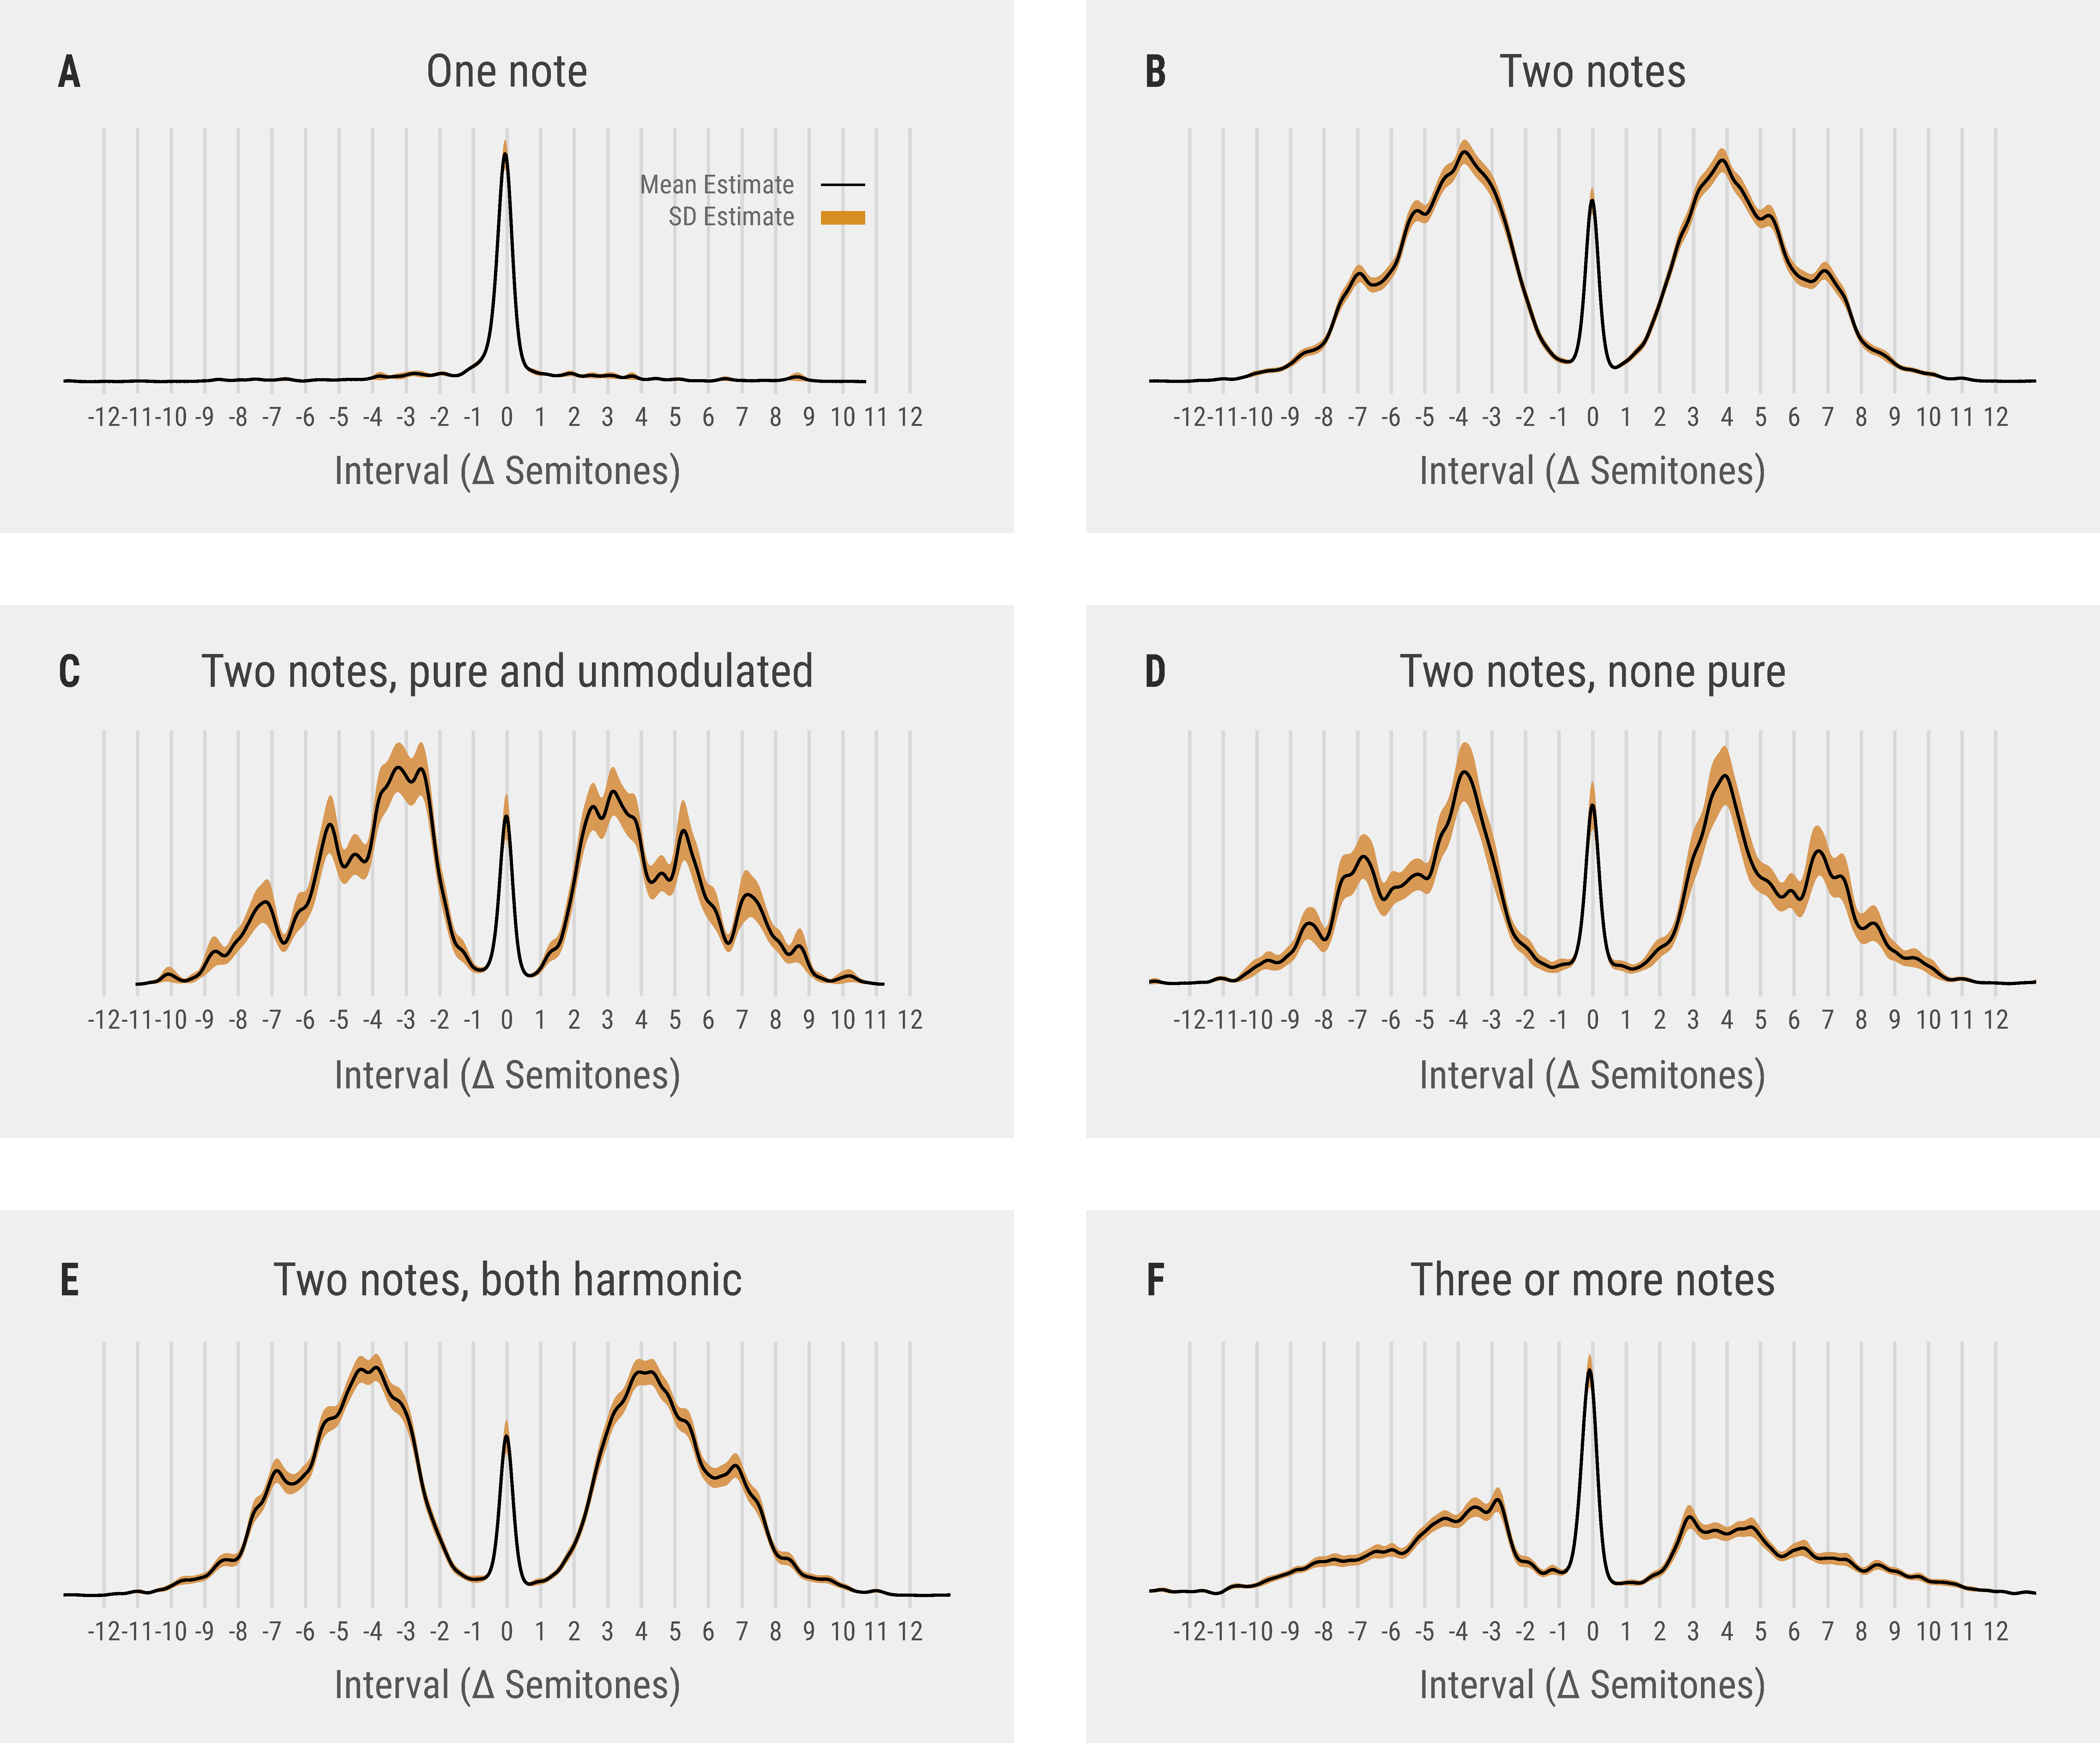
\includegraphics[width=\linewidth]{figures/chapter_5/melodic-songtypes.pdf}
    \mycaption{Kernel density estimates of the distribution of melodic intervals across a typology of songs}{
    In this figure, we categorise songs into distinct types based on the number of notes they contain and their spectral properties and plot the estimated density distribution of melodic intervals, measured in semitones and spanning the octave (ascending and descending).
    
    (A) One note: Songs consisting of a single note repeated rhythmically.
    (B) Two notes: All songs composed of two different, alternating notes.
    (C) Two notes, pure and unmodulated: Songs with two notes, each consisting of a single stable, pure, unmodulated tone.
    (D) Two notes, none pure: All two-note songs where neither note is pure and unmodulated.
    (E) Two notes, both harmonic: Songs featuring two notes, both of which have harmonic components.
    (F) Three or more notes: Songs comprising three or more notes. There are few three-note melodies, so we did not split these by spectral or modulation properties.
    }
    \label{c5_fig:melodic-songtypes}
\end{figure*}

\subsection{Melodic structure}

In a series of iterated learning experiments with humans, \textcite{anglada-tort2023} discovered that as melodies were learned and passed on, they acquired properties seen across human cultures \autocite{brown2013, mehr2019, savage2015}. In particular, they became biased towards a small vocabulary of intervals ($\le$7 categories, or 'peaks'), and used small interval sizes ($\le$7 semitones, or a perfect fifth). We now present evidence that the distribution of melodic intervals in the songs of our great tit population follows a highly structured pattern and shares these characteristics with human melodies and discuss some possible reasons for this convergence. (See \figref[a]{c5_fig:methods} and \autoref{c5_fig:melodic-songtypes}.)

\begin{table*}[hb!]
    \centering
    \mycaption{Name and size of intervals within the octave in the Western chromatic scale}{
    This table includes interval name, number of semitones, interval sizes measured in cents within equal temperament, corresponding frequency ratios with respect to just intonation, and the decimal values for those just intonation intervals in twelve-tone equal temperament (adapted from \cite{muller2016}).
    }
    \label{table:intervals}
    \begin{tblr}{
        colspec={X[l] X[c] X[c] X[c]},
        rowsep=2pt,
        stretch = 0.8,
        rowhead=1,
        row{odd} = {tablegrey},
        cells = {font = \fontsize{8pt}{8pt}\selectfont},
        row{1} = {tableheadgrey, font=\fontsize{8pt}{8pt}\selectfont\bfseries},
    }
    {Scale-Step Interval} & {Semitones} & {Equal Temp. (cents)} & {Ratio} & {12 \textsc{TET} value} \\
    Perfect Unison (U) & 0 & 0 & 1:1 & 1 \\
    Minor Second (m2) & 1  & 100  & 16:15 & 1.059463 \\
    Major Second (M2) & 2 & 200  & 9:8 & 1.122462 \\
    Minor Third (m3) & 3 &  300  & 6:5 & 1.189207 \\
    Major Third (M3) & 4 & 400 & 5:4 & 1.259921 \\
    Perfect Fourth (P4) & 5 & 500  & 4:3 & 1.33484 \\
    Tritone (T) & 6 &  600 & 64:45 & 1.414214 \\
    Perfect Fifth (P5) & 7 & 700  & 3:2 & 1.498307 \\
    Minor Sixth (m6) & 8  & 800  & 8:5 & 1.587401 \\
    Major Sixth (M6) & 9  & 900 & 5:3 & 1.681793 \\
    Minor Seventh (m7) & 10  & 1000  & 16:9 & 1.781797 \\
    Major Seventh (M7) & 11 & 1100  & 15:8 & 1.887749 \\
    Octave (P8) & 12 & 1200  & 2:1 & 2 \\
    \end{tblr}
\end{table*}

\subsubsection{Great tit songs favour small intervals}

The mean interval size observed in great tit songs from Wytham Woods was approximately 4.37 semitones (95\% CI [4.36, 4.38]). This falls in line with the interval sizes produced by human participants from India and the United States, which had a combined mean of 4.48 semitones (95\% CI [4.24, 4.72]). This pattern, which stands as one of the few true 'universals' in music, can be attributed to vocal range constraints: melodies transmitted orally tend to be biased toward small intervals, in contrast to those transmitted through other means or solely driven by preference \textcite{anglada-tort2023}. That the precise range is so similar to humans is interesting but presumably a coincidence driven by the particular vocal abilities of great tits. In contrast, a study analyzing melodic intervals in musician wrens \autocite{doolittle2012} found that the most common interval was the octave (12 semitones), which is extremely rare in great tits; and a comparison of 80 bird songs with human melodies showed that the latter have smaller average intervals on average \autocite{tierney2011a}. This difference might stem from the fact that some birds can execute large pitch jumps in their songs by independently adjusting tension in the labia of their bipartite syrinx \autocite{suthers2004}.

Interestingly, in the cross-cultural experiment by \textcite{anglada-tort2023}, melodic intervals produced by Indian participants were significantly smaller (3.25 [2.93, 3.57] semitones on average, 95\% CI) than those produced by US participants (5.71 [5.55, 5.86] semitones). This aligns with corpus studies showing that intervals in Carnatic melodies are smaller than those in Western melodies \autocite{bowling2012} and suggests that, even within the range dictated by motor-vocal constraints, cultural influences can shape the overall distribution of interval sizes in human music. As for great tits, we cannot definitively conclude whether variation in average interval sizes is similarly influenced by cultural factors, simply because our dataset, while comprehensive, is derived from a single population. We present qualitative evidence that, despite the high turnover in great tit songs due to population turnover and other demographic processes (as discussed in the previous chapter), the overall distribution of interval sizes remains remarkably stable across three consecutive years (see \autoref{c5_fig:melodic-byyear}).

\paragraph{Skip-reversal patterns}
In order to further characterise the general melodic structure of great tit songs, we plot the interval size in semitones as a function of the interval's starting frequency in \figref[c]{c5_fig:methods}. This reveals a very strong pattern known as 'skip-reversal', where larger intervals are associated with extreme pitches---a phenomenon that has stirred debate in musicology quarters \autocite{vonhippel2000} but likely arises from a simple process of regression to the mean due to motor constraints. In essence, when a melody approaches the boundaries of the singer's comfortable vocal range, also known as the 'tessitura,' it has little choice but to return toward the centre of the range \autocite{tierney2008, vonhippel2000, vonhippel2000a}. 



\subsubsection{Melodic intervals are categorically organised}
As we have seen, great tit songs predominantly feature small melodic intervals, which can likely be attributed to motor-vocal constraints. Next, we want to determine if the distribution of interval sizes within the vocal range of great tits is different from what we would expect by chance. To find out, we created a null distribution by shuffling the empirical distribution of frequencies and recalculating interval sizes. This null distribution represents what we would expect if birds with the same vocal range had no preference for specific interval sizes (shown as the grey discontinuous line in \figref[b]{c5_fig:methods}). Simply due to the unimodal shape of the distribution of note frequencies sung by great tits (mean frequency: 4310.05 Hz, SD: 926.5; \figref[c]{c5_fig:methods}, top panel), interval sizes in this null distribution are centred around zero. Though perhaps naive---due to communicative and perceptual pressures, we might expect birds to avoid barely perceptible changes, for example---this comparison allows us to see that the empirical distribution of melodic intervals is highly structured, and it is so in interesting ways. \autoref{c5_fig:melodic-songtypes} presents the probability density distribution estimated for each set of songs in our typology.


\paragraph{One-note songs} 
The one-note case in \figref[a]{c5_fig:melodic-songtypes} is, by definition, tightly clustered around the unison (0 semitones), and gives a good idea of the population-level variance found when birds are trying to repeat the same note consistently.

\begin{figure*}[ht!]
    \centering
    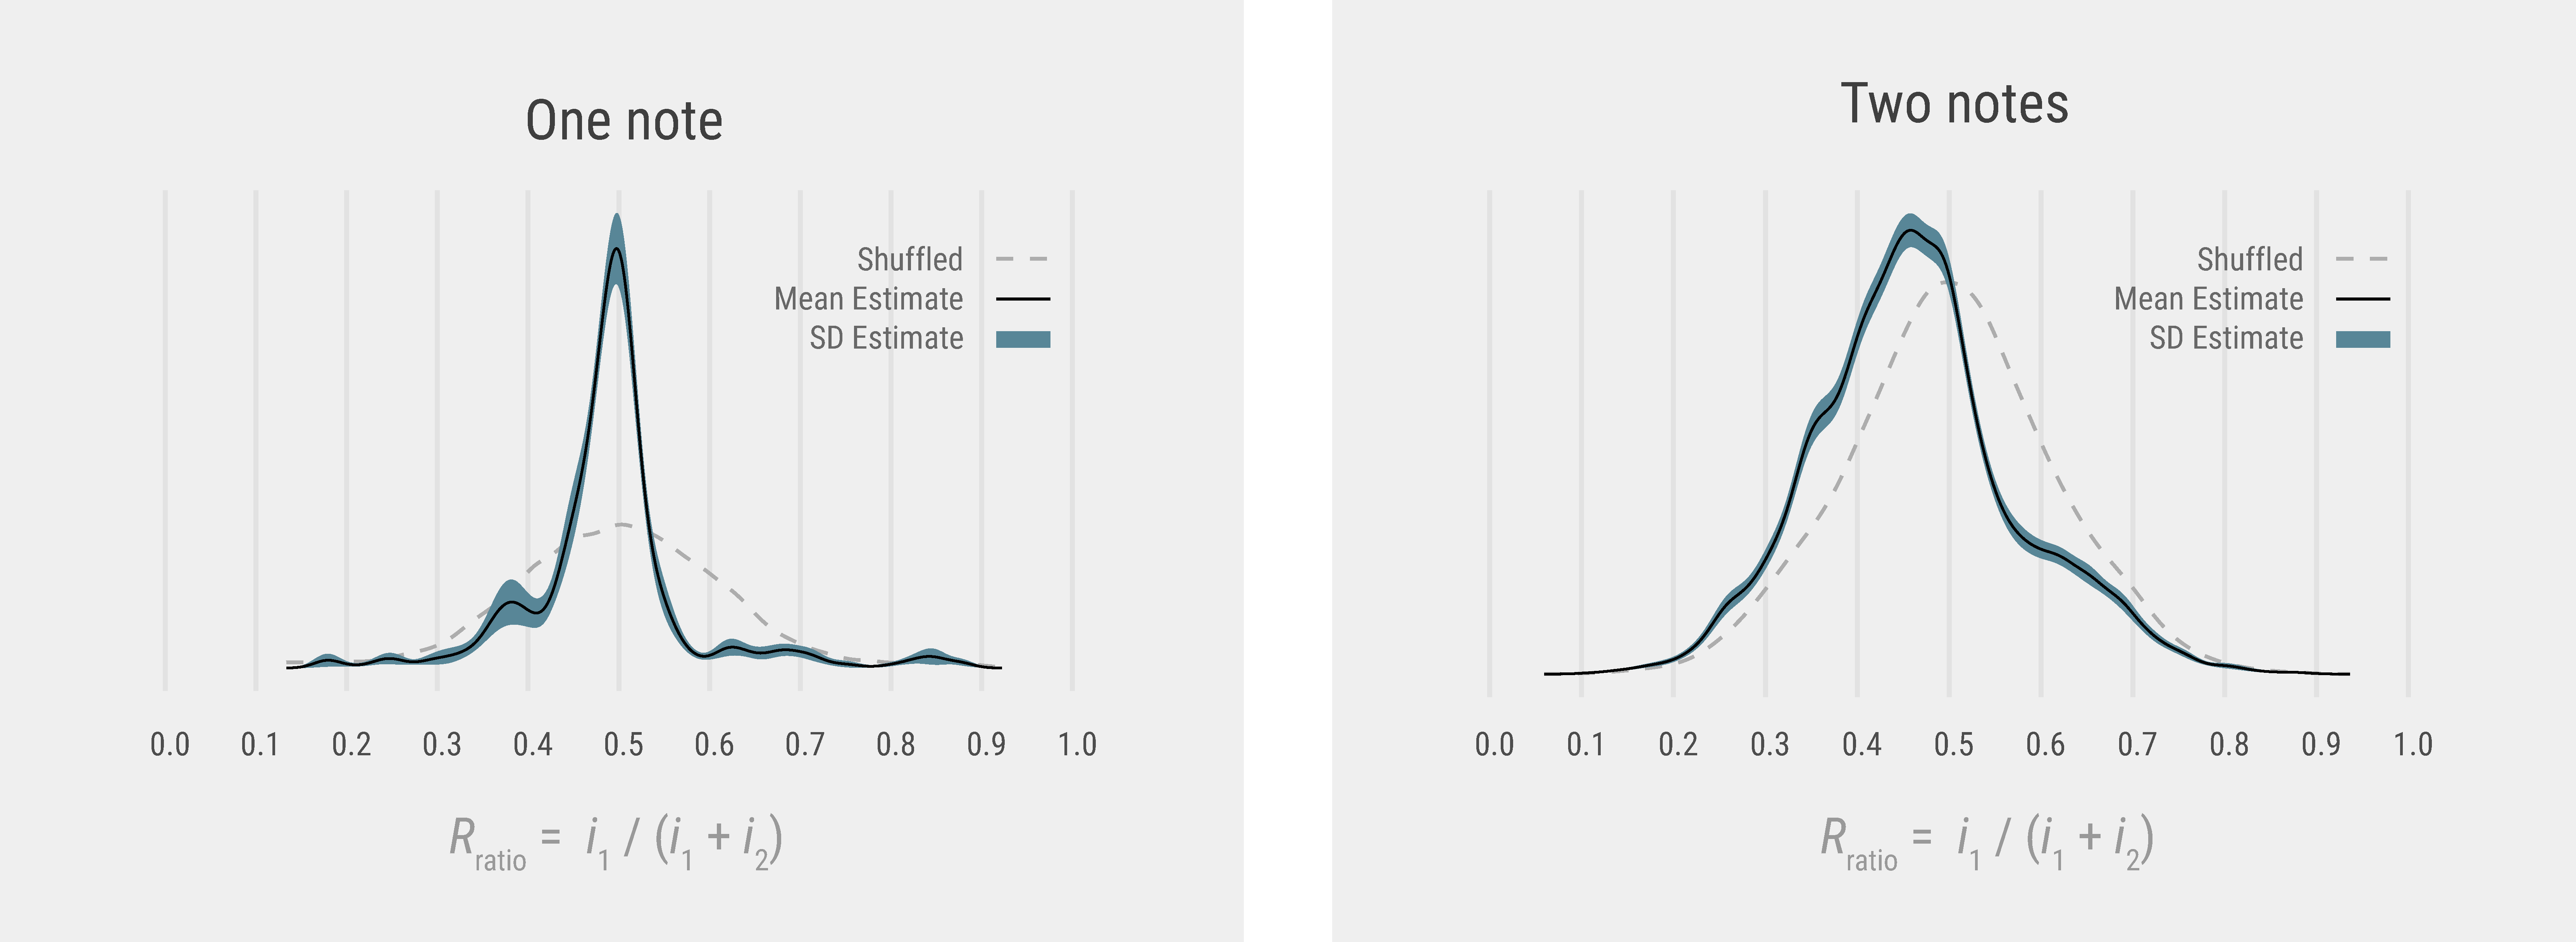
\includegraphics[width=\linewidth]{figures/chapter_5/rhythmic-nulls.pdf}
    \mycaption{Rhythmic ratios in one and two-note songs}{
    Density estimate of the distribution of rhythmic ratios in one-note (left) and two-note songs (right), with mean (black line) and SD (orange line). The discontinuous grey line represents a null distribution created by shuffling the empirical distribution of inter-onset intervals and recalculating interval sizes.
    }
    \label{c5_fig:rhythmic-nulls}
\end{figure*}


\paragraph{Songs with multiple notes}
In cases where birds sing melodies with two or more notes (\figref[b-f]{c5_fig:melodic-songtypes}), we observe a noticeable dip in the smallest intervals (less than 2 semitones). This suggests that birds strongly avoid melodies with very small frequency changes. Interestingly, this pattern resembles what we find in human songs, where it's interpreted as a result of perceptual preferences \autocite{bowling2012, kuroyanagi2019}. However, it could also relate to production difficulties, as very small intervals might be harder to sing accurately than unisons or larger leaps \autocite{anglada-tort2023}.

The rest of the distribution also exhibits non-random features. It reveals evidence of potential melodic interval categories, defined as local maxima or modes. These patterns may be driven by a preference for certain interval sizes or interval ratios, a phenomenon observed in human music, or other, currently unknown processes. Some melodic intervals produced by great tits in our population cluster around specific interval categories commonly found in human music; these include intervals of 7 and 4 semitones, both ascending and descending, which correspond to what is considered the most consonant interval within the octave (\href{https://en.wikipedia.org/wiki/Perfect_fifth}{perfect fifth}, 3:2) and the \href{https://upload.wikimedia.org/wikipedia/commons/transcoded/2/2a/Just_major_third_on_C.mid/Just_major_third_on_C.mid.mp3}{major third}, respectively. See \autoref{table:intervals}. The latter, which in the harmonic series would correspond to the interval between the fourth and fifth harmonics, is the most common interval size in great tit songs.

We also see a peak around 5.2 semitones in the simpler (two-note, pure, unmodulated) songs \figref[c]{c5_fig:melodic-songtypes} which is not present in \figref[d--f]{c5_fig:melodic-songtypes}. The difference in the exact location of these peaks across the typology of songs might reflect an interaction between song syntax or production and interval categories, or, as discussed in the \autoref{c5:strength}, less precise measurement due to the spectral complexity of notes.

It is fascinating to consider the possibility that similar perceptual, cognitive, and production biases might shape the interval structure in both great tit and human melodies. However, even if the alignment of interval categories is coincidental, the presence of a limited number of modes (at $\approx$7, $\approx$5.2, $\approx$4, and $\approx$0 semitones; ascending and descending) within a comprehensive dataset of songs representing distinct song types that undergo rapid turnover, suggests that melodic structure does not merely evolve randomly due to copying errors. Instead, it raises the possibility that interval categories play a role in stabilising and anchoring cultural variation, much like they do in human melodies. More generally, there is evidence that the emergence of shared categories in an otherwise graded or continuous trait space facilitates efficient and accurate transmission  \autocite{falandays2022, tchernichovski2017, silvey2019, decastro-arrazola2019, kirby2017}, and we believe that a similar process might drive the patterns in our data.

From our multi-year dataset, we observe that the exact positions of interval categories are relatively stable, although not as much as the broader shape of the distribution (two main modes and a trough between them, \autoref{c5_fig:melodic-byyear}). However, adequately testing whether these fine-scale melodic biases can also shift due to cultural evolutionary processes will require longer-term data or data from a wider geographic region.


\begin{figure*}[ht!]
    \centering
    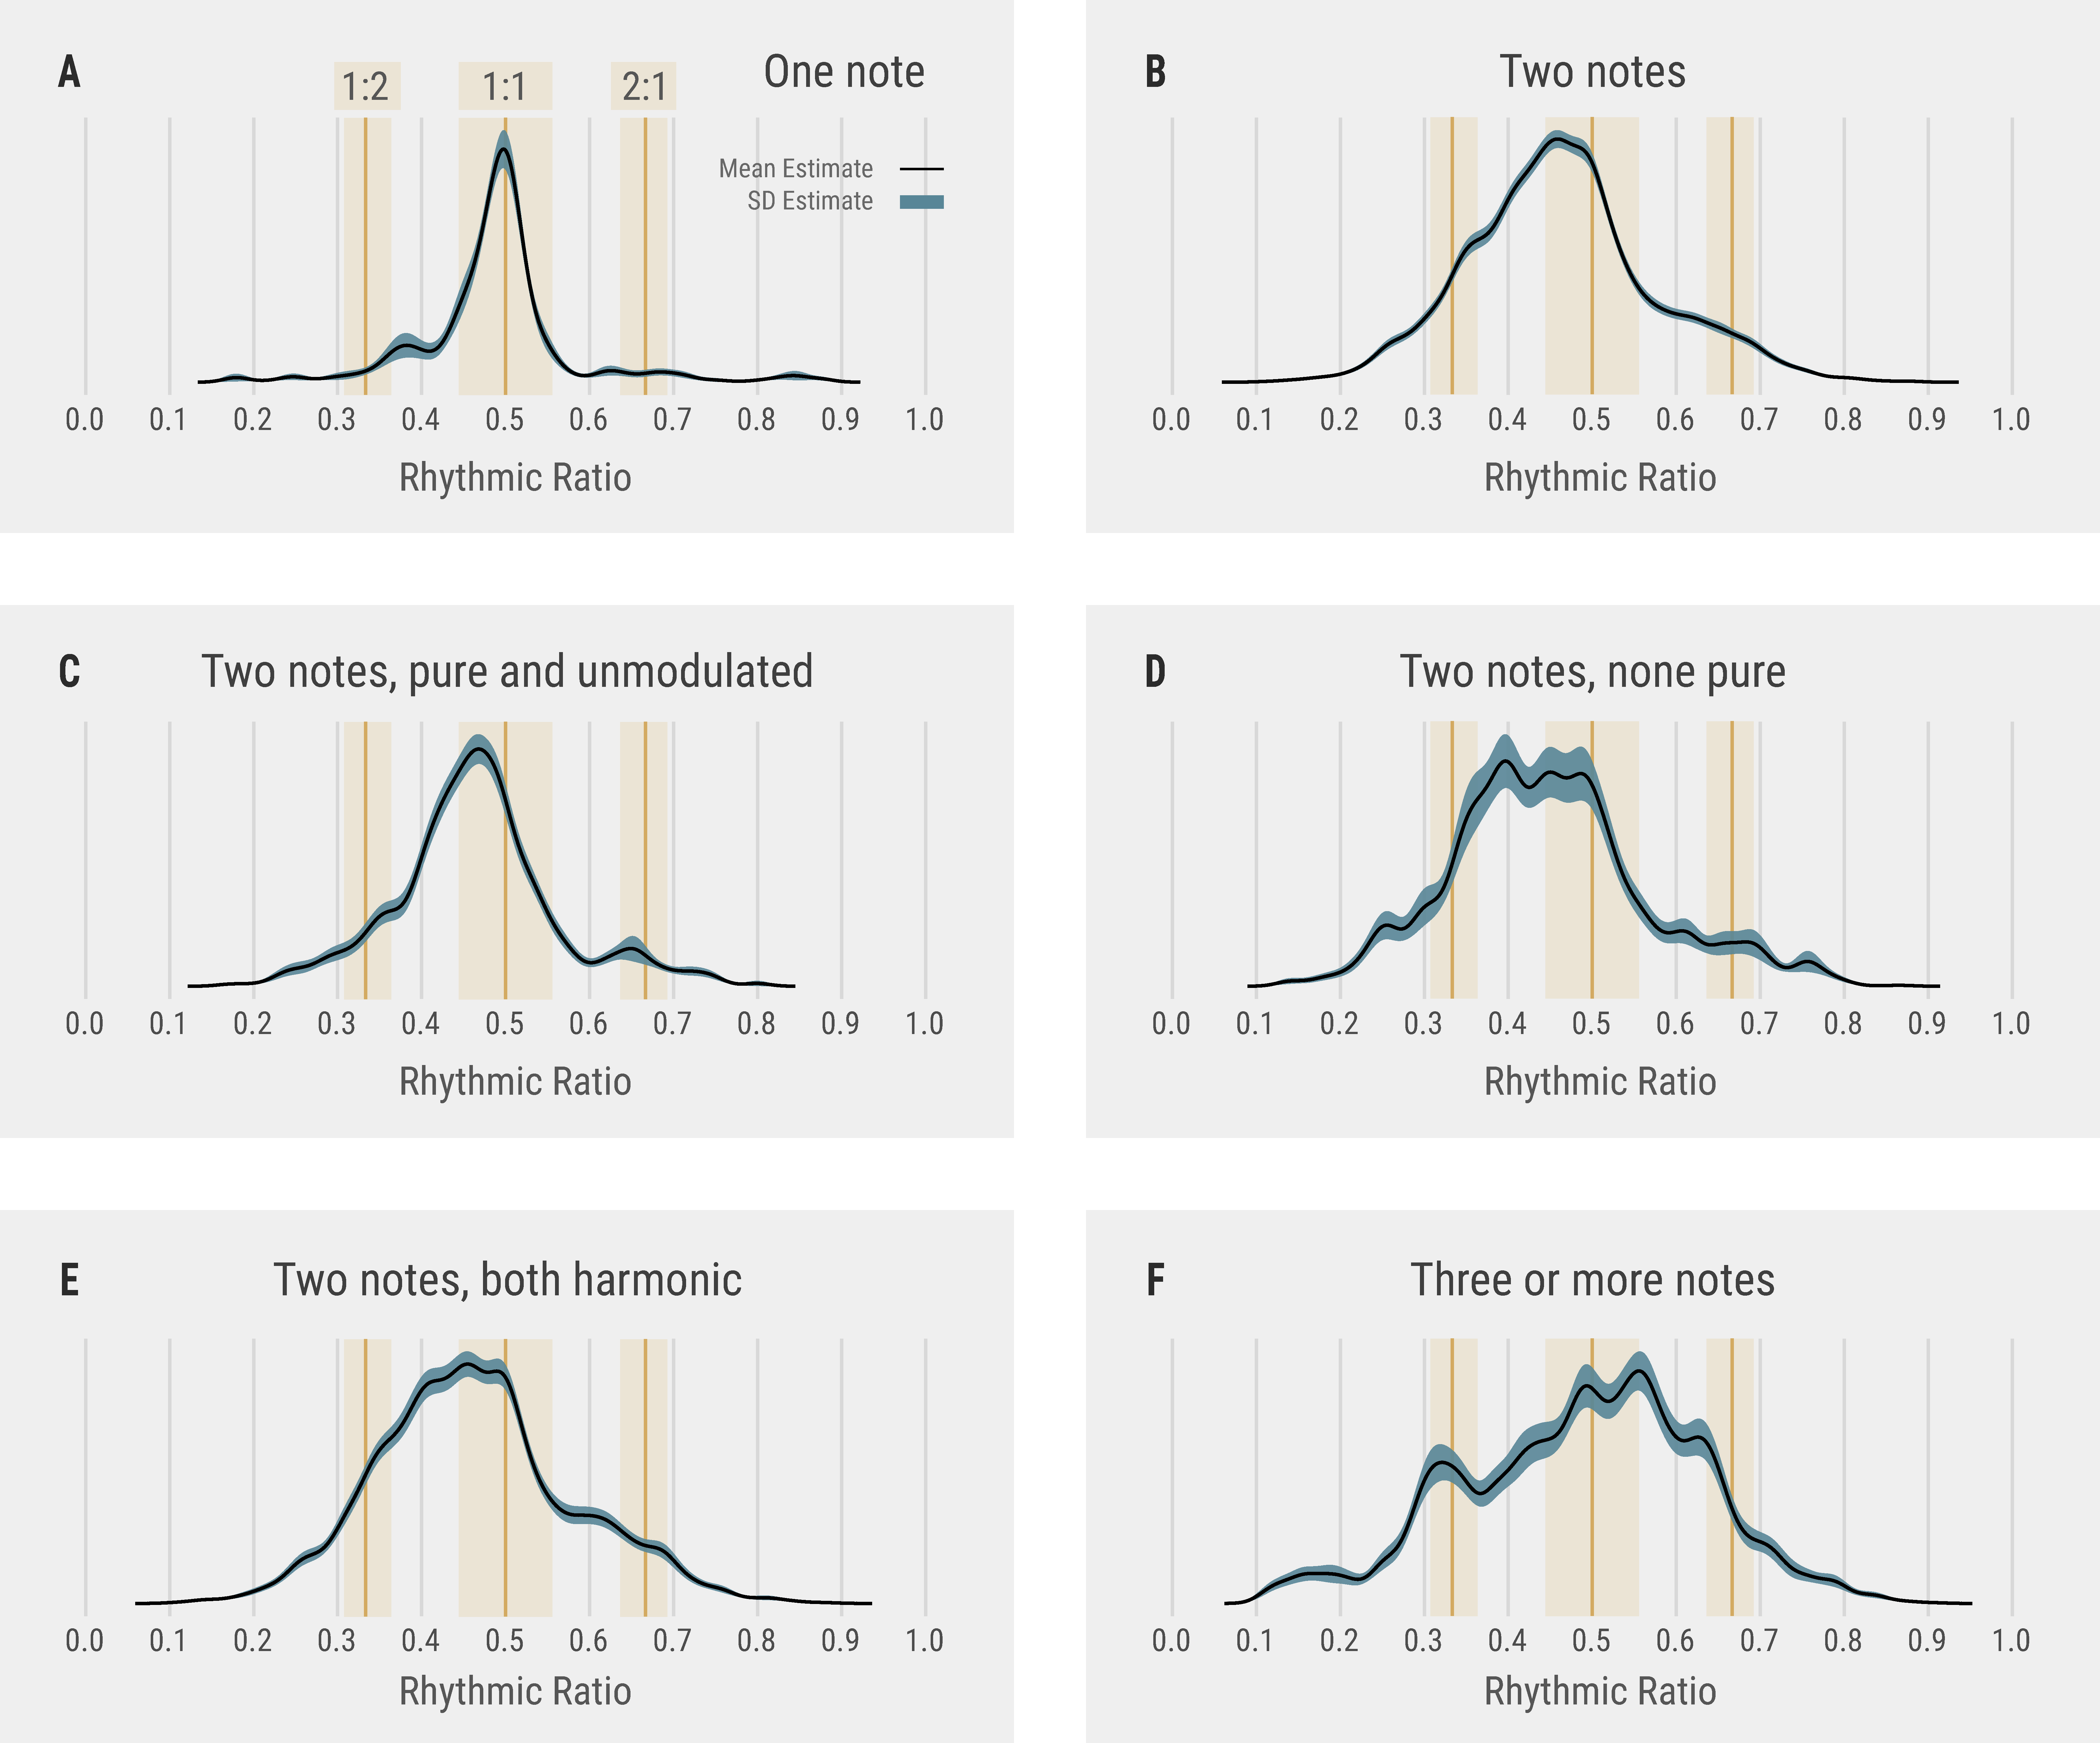
\includegraphics[width=\linewidth]{figures/chapter_5/rhythmic-songtypes.pdf}
    \mycaption{Kernel density estimates of the distribution of rhythmic ratios across a typology of songs}{
    We categorise songs into distinct types based on the number of notes they contain and their spectral properties and plot the estimated density distribution of rhythmic ratios, calculated as the ratio of the first inter-onset interval to the sum of the first and the second. Orange vertical lines and shaded areas represent, from left to right 1:2, 1:1, and 2:1 rhythms, and the 'on-integer' ranges as per \textcite{degregorio2021, roeske2020}

    }
    \label{c5_fig:rhythmic-songtypes}
\end{figure*}


\subsection{Rhythmic structure}

Rhythmic patterns in songs are constructed by the temporal intervals between note onsets and can be broadly categorised into periodic or aperiodic. Periodic or repeating patterns can further be divided into isochronous---where a single interval, say, 0.5 seconds, is consistently repeated---and heterochronous, where intervals vary in duration. Heterochronous patterns, in turn, can be described by small integers (like 1:2) or more complex ratios (e.g., 16:23). In human music, rhythms often employ ratios such as 1:2, 1:3, and 2:3 but avoid ratios like 31:8 \autocite{ravignani2014}. Regular or isochronous patterns are a pervasive feature of musical rhythm, often attributed to the need for group coherence and predictability in collective performance and dancing \autocite{kotz2018}. 

Furthermore, cross-cultural experiments have shed light on the prevalence of specific rhythmic templates across different societies. 1:1 and 2:1 rhythmic templates are widespread across cultures, while more complex ratio categories, such as 3:2 and 4:3, are influenced by cultural trajectories and exposure \autocite{polak2018, jacoby2017a, jacoby2021}. Combined with other laboratory experiments \autocite{ravignani2017a} showing how these can emerge from random stimuli and enhance how accurately participants can reproduce them, this may indicate that these categories emerge, at least in part, during learning and cultural transmission and serve to stabilise it.

\subsubsection{Rhythmic abilities in other species}
While the focus of most research on rhythm has rested with human music, there is increasing evidence that other animal species can both produce and discern regular rhythms \autocite{rouse2021, verga2022, vanderaa2015}. For example, zebra finches, thrush nightingales, rock hyraxes \textit{Procavia capensis}, and various singing primates have demonstrated isochronous rhythm production \autocite{roeske2020, norton2016, demartsev2023, degregorio2021, degregorio2023, raimondi2023}. This suggests that more fundamental, widespread motor or perceptual processes may underlie these rhythmic abilities. Integer ratio rhythms might be more easily produced, for example, or representational constraints could affect perception and make categories characterised by simple mathematical relationships more likely to arise \autocite{ravignani2018c, roeske2020, jacoby2017a}.


\subsubsection{Exploring Rhythmic Structure in Great Tit Songs}

In this context, we examine the rhythmic structure of great tit songs. Similar to our approach with melodies, we compare the empirical distribution of rhythmic ratios with a null distribution obtained by shuffling the observed range of inter-onset intervals (the time between consecutive note onsets) and recalculating the ratios between them. The analysis reveals that rhythm in great tit songs is generally biased towards isochrony (\autoref{c5_fig:rhythmic-nulls}). We also investigate whether rhythmic structure remains invariant when considering other song properties, such as the number of notes in a phrase. Our findings suggest that rhythm interacts with syntax or melodic structure, as it is not consistent across all song types \autocite{xing2022}.

\paragraph{One-note songs}
For instance, the distribution of one-note songs (0 semitone intervals) is strongly organised around isochronic rhythms (identical intervals, 1:1 ratio), as evidenced by a steeply unimodal distribution perfectly centred around 0.5 in \figref[a]{c5_fig:rhythmic-songtypes}. This finding contributes to a small but growing body of evidence of this universal characteristic of human music in other species \autocite{xing2022, rouse2021, roeske2020, demartsev2023, degregorio2021, degregorio2023, raimondi2023}. Indeed, we speculate that as more instances of isochrony in animal vocalisations are discovered, exceptions may become more intriguing than the norm.

\paragraph{Two-note songs}
As summarised in \figref[b]{c5_fig:rhythmic-songtypes}, two-note songs also have a unimodal distribution of rhythmic ratios, with more variance. Interestingly, they deviate slightly from a perfect isochronous pattern, with the first interval being slightly shorter than the second. This pattern is reminiscent of patterns observed in Indris lemurs \autocite{degregorio2021} and Australian pied butcherbirds (personal observation from \cite{xing2022}). We believe there are two possible explanations for this deviation: motor constraints due to producing alternating frequencies that are not present in the single-note phrases, or a more complex, perceptually-mediated departure from expectations for aesthetic purposes, akin to 'tempo rubato' \autocite{parncutt1994, degregorio2021} or 'backbeat delay' in music \autocite{frane2017}.

\paragraph{Songs with more than two notes}
In songs that feature more than two alternating notes, the rhythmic landscape becomes more complex. Peaks emerge around isochrony (1:1) and a $\approx$ 1:2 ratio, along with other, more complex rhythms. When great tits produce three-interval rhythms, our analysis reveals distinctive modes near the two smallest integer ratios, which are widely prevalent in human music performances and traditions \autocite{jacoby2017a, jacoby2021}. This, which has also been found in thrush nightingales and indris \autocite{roeske2020, degregorio2021}, is again strongly suggestive of common motor, cognitive, or perceptual biases across vocalising species.

\section{Conclusion} 

In this study, we examine the melodic and rhythmic structure of great tit songs and find similarities with human songs and those of other birds and mammals. Our analysis of melodic structure reveals that great tit songs favour small intervals, likely due to vocal range constraints. The distribution of these intervals is highly non-random: it exhibits distinct modes that align closely with interval sizes commonly found in human music. Similarly, our analysis of rhythmic structure in great tit songs uncovers categorical organisation. Some song types feature precisely timed, isochronous rhythms, while others exhibit more dynamic patterns with varying inter-note intervals.

In summary, our study underscores the presence of strong structural biases in both the melody and rhythm of great tit songs. These biases likely result from a combination of motor and cognitive or perceptual processes that come into play during the learning and transmission of songs. In the previous chapter, we saw that song turnover in great tits was high, driven by high population turnover and other demographic processes. However, despite the rapid introduction and loss of new cultural variants, cultural similarity and consistency remain high. Given the relative simplicity of these songs, the non-random variation in their melodic and rhythmic foundations likely contributes significantly to their stability and cultural fidelity. Future research will expand upon these findings by exploring these patterns in a broader geographic context and over more extended periods, providing insights into the intrinsic mechanisms governing cultural diversity and evolution in avian vocalisations.

\section{Data and code}

The code to replicate these analyses and figures can be found at \href{https://github.com/nilomr/greti-song-intervals}{\nolinkurl{github/nilomr/greti-song-intervals}}. All the data are available from \href{https://osf.io/n8ac9}{osf.io/n8ac9}, and documented \href{https://nilomr.github.io/great-tit-hits/}{here}.

\section{Acknowledgements}
This is a very early draft of this work, and many analyses remain to be run. Be advised that it probably contains a few blunders. We thank the members of the Computational Auditory Perception group at the Max Planck Institute for Empirical Aesthetic, Andrea Estandía, Carys Jones, and especially Manuel Anglada-Tort for a very useful discussion of preliminary ideas and results around this work. We also thank all those who have contributed to the long-term nest box study in Wytham Woods and the collection of associated data. This work was supported by a Clarendon-Mary Frances Wagley Graduate Scholarship and an EGI scholarship to Nilo Merino Recalde, and made use of the University of Oxford Advanced Research Computing facility \parencite{richards2015}.

\section{Author contributions}

\textbf{Nilo Merino Recalde}: Conceptualization, Methodology, Software, Formal analysis, Investigation, Data Curation, Writing - Original Draft, Writing - Review \& Editing, Visualization. 
\textbf{Ben C. Sheldon}: Supervision, Project administration, Writing -- review and editing, Funding acquisition.

\renewcommand{\cleardoublepage}{}
\renewcommand{\clearpage}{}
\printbibliography

% %\onecolumn % start one-column layout for chatper 4 - supplementary
% send to new page
\renewcommand{\cleardoublepage}{}
\renewcommand{\clearpage}{}
\supplementarysection
\noindent (Next page)

\begin{figure*}
    \centering
    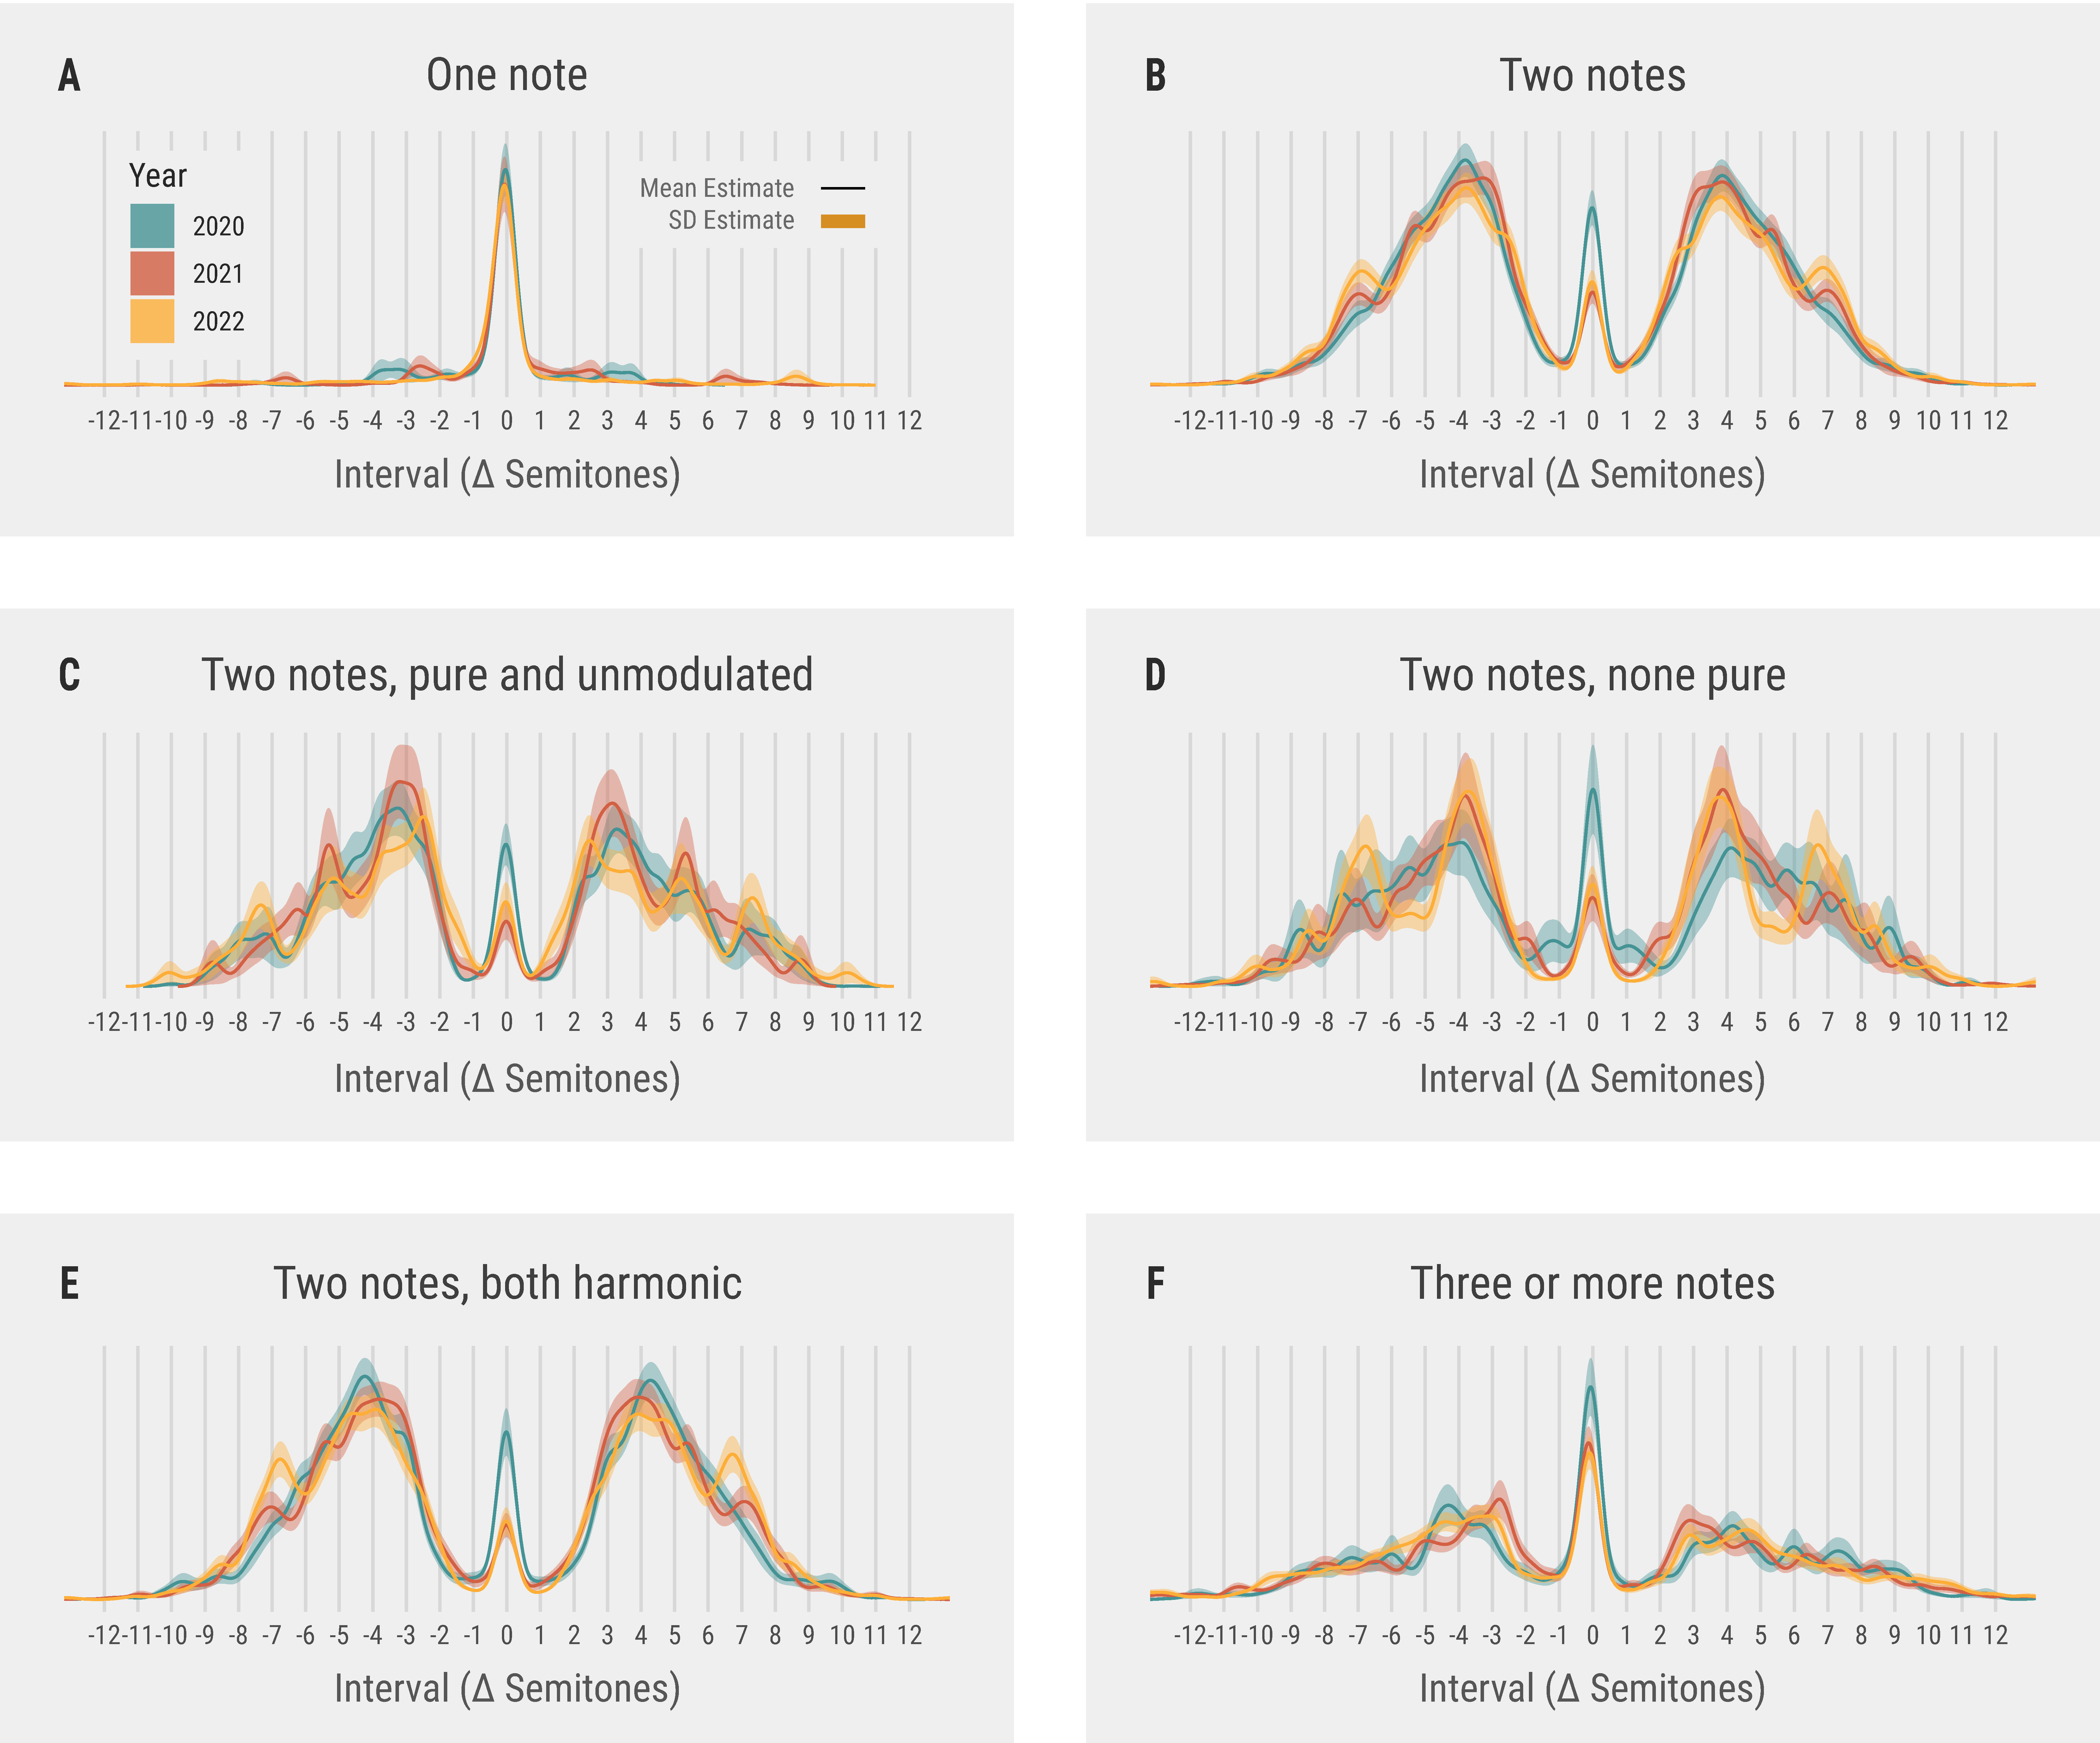
\includegraphics[width=\linewidth]{figures/chapter_5/melodic-songtypes-byyear.pdf}
    \mycaption{Kernel density estimates of the distribution of melodic intervals across a typology of songs in different years}{
    In this figure, we categorise songs into distinct types based on the number of notes they contain and their spectral properties and plot the estimated density distribution of melodic intervals, measured in semitones and spanning the octave (ascending and descending). Colours represent separate years in our study. 
    
    (A) One note: Songs consisting of a single note repeated rhythmically.
    (B) Two notes: All songs composed of two different, alternating notes.
    (C) Two notes, pure and unmodulated: Songs with two notes, each consisting of a single stable, pure, unmodulated tone.
    (D) Two notes, none pure: All two-note songs where neither note is pure and unmodulated.
    (E) Two notes, both harmonic: Songs featuring two notes, both of which have harmonic components.
    (F) Three or more notes: Songs comprising three or more notes. There are few three-note melodies, so we did not split these by spectral or modulation properties.
    }
    \label{c5_fig:melodic-byyear}
\end{figure*}

